\documentclass{report}
\usepackage[T1]{fontenc} % Fontes T1
\usepackage[utf8]{inputenc} % Input UTF8
%\usepackage[backend=biber, style=ieee]{biblatex} % para usar bibliografia
%\usepackage{csquotes}
\usepackage[portuguese]{babel} %Usar língua portuguesa
\usepackage{blindtext} % Gerar texto automaticamente
\usepackage[printonlyused]{acronym}
\usepackage{hyperref} % para autoref
\usepackage{graphicx}
\usepackage{listings}
\usepackage{float}

%\bibliography{bibliografia}
\renewcommand{\labelitemii}{$\star$}


\begin{document}
%%
% Definições
%
\def\titulo{Projecto 2}
\def\data{15 de junho de 2018}
\def\autores{Rodrigo Rosmaninho, Eurico Dias,\\ João Trindade, Pedro Valério}
\def\autorescontactos{(88802) r.rosmaninho@ua.pt, (72783) dias.eurico@ua.pt,\\ (89140) jatt@ua.pt, (88734) pedrovalerio@ua.pt}
\def\versao{Versão 1}
\def\departamento{Departamento de Eletrónica, Telecomunicações e Informática}
\def\empresa{Universidade de Aveiro}
\def\logotipo{ua.pdf}
%
%%%%%% CAPA %%%%%%
%
\begin{titlepage}

	\begin{center}
		%
		\vspace*{50mm}
		%
		{\Huge \titulo}\\
		%
		\vspace{10mm}
		%
		{\Large \empresa}\\
		%
		\vspace{10mm}
		%
		{\LARGE \autores}\\
		%
		\vspace{30mm}
		%
		\begin{figure}[h]
			\center
			\includegraphics{\logotipo}
		\end{figure}
		%
		\vspace{30mm}
	\end{center}
	%
	\begin{flushright}
		\versao
	\end{flushright}
\end{titlepage}

%%  Página de Título %%
\title{%
{\Huge\textbf{\titulo}}\\
{\Large \departamento\\ \empresa}
}
%
\author{%
	\autores \\
	\autorescontactos
}
%
\date{\data}
%
\maketitle

\pagenumbering{roman}

\tableofcontents
% \listoftables     % descomentar se necessário
\listoffigures


%%%%%%%%%%%%%%%%%%%%%%%%%%%%%%%
\clearpage
\pagenumbering{arabic}

%%%%%%%%%%%%%%%%%%%%%%%%%%%%%%%%
\chapter{Introdução}
\label{chap.introducao}

O presente relatório foi elaborado com o propósito de descrever e analisar a elaboração e resultado do segundo projecto realizado no âmbito da unidade curricular de Laboratórios de Informática. Iniciando-se com uma apresentação do tema proposto, segue-se a estrutura do documento separada por capítulos representativos das componentes fundamentais do projecto desenvolvido.

O objectivo do projecto realizado foi a elaboração de um sistema que permite a composiçao de músicas com recurso a excertos de áudio, disponível através de um interface web. Este interface permite compôr músicas, ouvir composições de outras pessoas, carregar excertos para serem utilizados e descarregar músicas criadas. A informação de todas as músicas e excertos devem encontrar-se registados numa base de dados, que permita o acesso e modificação dos dados armazenados. A criação de músicas deve ser possível através de um programa gerador de excertos áudio, conforme a informação recebida sobre o tipo de música a criar.

Este documento encontra-se dividido em capítulos e secções descritivas das componentes referidas, sendo este o seu primeiro capítulo. No \autoref{chap.web}, é descrito em detalhe o interface web criado, sendo as suas páginas explicadas separadamente, na \autoref{sec.songlist}, \autoref{sec.samplist} e \autoref{sec.create}. No \autoref{chap.api}, é explicada a implementação da aplicação web e a forma como se interliga com os restantes componentes. No \autoref{chap.db}, apresenta-se a organização do sistema de base de dados, bem como as suas funcionalidades. No \autoref{chap.audio} é explicado o processo de criação de excertos musicais com base numa pauta num formato de dicionário, sendo o seu processo descrito em \autoref{sec.pauta}, \autoref{sec.efeitos}, \autoref{sec.comp} e \autoref{sec.escrita}. Por último, no \autoref{chap.conclusao}, são apresentadas as conclusões do trabalho.

%Nota: Adicionar gerador de imagens e análise de resultados de conveniente.
%Nota: Adicionar as secções e subsecções dos restantes capítulos, caso existam.

\chapter{Interface Web}
\label{chap.web}

Em todas as páginas é possível alterar o avatar (foto) do utilizador clicando no seu nome no canto superior direito.\\
Nota: Em todas as páginas foi utilizado o Twitter Bootstrap (versão 4)

\section{Lista de Músicas}
\label{sec.songlist}

A primeira página consiste numa lista de todas as músicas criadas até ao momento.
As funcionalidades dinâmicas desta página são fornecidas pelo ficheiro \textbf{songlist.js}

A listagem é conseguida através de uma chamada ao endpoint \textbf{list/?type=songs},
que devolve um objeto JSON com um array de todas as músicas presentes no sistema. Por exemplo:\\

\begin{lstlisting}
    [
        {
          "name": "teste",
          "id": "8434efc3978369c2",
          "date": "2018-06-13 21:29:23Z23.227",
          "uses": 0,
          "path": "songs/8434efc3978369c2.wav",
          "votes": 1,
          "author": "r.rosmaninho"
        },
        {
          "name": "teste 2",
          "id": "4cc7daf0c5bc921a",
          "date": "2018-06-15 17:13:29Z29.465",
          "uses": 0,
          "path": "songs/4cc7daf0c5bc921a.wav",
          "votes": 0,
          "author": "r.rosmaninho"
        }
      ]
\end{lstlisting}

A informação de cada lista é depois adicionada à tabela presente em \textbf{songs.html} \\

\begin{figure}[H]
	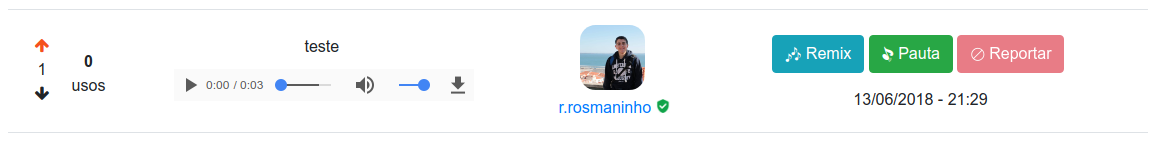
\includegraphics[scale=0.35]{song_list_item.png}
	\caption{Aspeto de um item da tabela}
	\label{img.song_list_item}
\end{figure}

É permitido ao utilizador votar na musica através de dois botões em forma de seta (um "para cima" e outro "para baixo").
Como se pode ver, as setas ficam coloridas para indicar que o utilizador já votou. 
Este processo acontece automáticamente a cada vez que o utilizador abre o website, necessitando, para isso, de receber informação sobre os votos efetuados pelo utilizador (proveniente da base de dados). \\

Para além das operações de voto, é ainda possível:

\begin{itemize}
  \item Visualizar o número de usos (vezes que a música foi utilizada para gerar outras músicas).
  \item Visualizar o nome da música (escolhido pelo utilizador que a criou).
  \item Reproduzir e descarregar a música (através da tag \textit{audio} do HTML). A música encontra-se armazenada no sistema de ficheiros da aplicação Web e é servida pelo \textbf{CherryPy}
  \item Visualizar o email (sem @ua.pt) do autor da música e o seu avatar. Se o autor fizer parte da equipa de desenvolvimento do website aparece um símbolo indicativo. Para além disso, é possivel passar o rato pelo nome para visualizar o \textit{karma} do autor (total de upvotes + downvotes)
  \item Visualizar a data e hora (em UTC) da criação da música.
  \item Fazer \textit{Remix} da música em questão (Alterar uma música existente e guardá-la como uma nova música). O utilizador é redirecionado para a página de criação de músicas, que é pre-populada com a pauta da música em questão
  \item Descarregar uma imagem representativa da pauta da música em questão em formato \textit{.png} através do botão \textit{Pauta}
  \item Reportar uma música à equipa de desenvolvimento (por linguagem inapropriada no título da música por exemplo). Esta ação adiciona uma entrada na tabela \textit{reports} da base de dados. Não é possível reportar músicas da autoria de um membro da equipa.\\
\end{itemize}

É possivel ordenar a lista por nome da música, data de criação, número de votos, e escolher entre ordem ascendente ou descendente. Ao escolher um novo tipo de ordenação a página é recarragada com os seguintes parametros (por exemplo):
\begin{lstlisting}
  /songs?order=votos&asc_desc=1
\end{lstlisting}
Pelo que o JavaScript faz o \textit{request} da lista ao API de forma diferente \\

A lista das músicas é apresentada de forma paginada. Apenas 10 músicas são apresentadas por página. As restantes ficam com o estilo \textbf{display: none;}. Este comportamento é gerido pelo JavaScript em \textbf{songlist.js} e é importante notar que \href{https://jsfiddle.net/solodev/yw7y4wez/}{este recurso externo} foi usado como inspiração.

\section{Lista de Excertos}
\label{sec.samplist}

A segunda página consiste numa lista de todos os excertos (samples) presentes no sistema até ao momento.
As funcionalidades dinâmicas desta página são fornecidas pelo ficheiro \textbf{sampleslist.js}

Tal como na página de músicas, a listagem é conseguida através de uma chamada a um endpoint do api. Neste caso \textbf{list/?type=samples},
que devolve um objeto JSON com um array de todos os excertos presentes no sistema. O objeto correspondente a cada elemento é extremamente semelhante ao que foi visto na \autoref{sec.songlist}:\\

A informação de cada lista é depois adicionada à tabela presente em \textbf{samples.html} \\

\begin{figure}[H]
	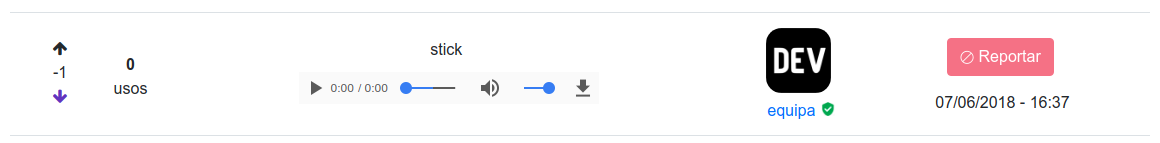
\includegraphics[scale=0.35]{sample_list_item.png}
	\caption{Aspeto de um item da tabela}
	\label{img.sample_list_item}
\end{figure}

Qualquer utilizador pode fazer upload de um novo excerto para a aplicação utilizando o \textit{form} HTML disponível para o efeito.
Apenas são aceites excertos em formato \textbf{.wav} e se o ficheiro for do tipo \textit{stereo} é automaticamente convertido para \textit{mono} com a ajuda do comando bash \textit{ffmpeg}
No backend é feito o hash do conteúdo do ficheiro e a informação é guardada na base de dados.\\

Mais uma vez, é permitido ao utilizador votar no excerto através dos dois botões em forma de seta. \\

Para além destas operações, é ainda possível:

\begin{itemize}
  \item Visualizar o número de usos (vezes que o excerto foi utilizado para gerar novas músicas).
  \item Visualizar o nome do excerto (escolhido pelo utilizador que fez o upload).
  \item Reproduzir e descarregar o excerto (através da tag \textit{audio} do HTML). O excerto também se encontra armazenado no sistema de ficheiros da aplicação Web e é servido pelo \textbf{CherryPy}
  \item Visualizar o email (sem @ua.pt) do utilizador que fez upload e o seu avatar. Se o autor fizer parte da equipa de desenvolvimento do website aparece um símbolo indicativo. Para além disso, é possivel passar o rato pelo nome para visualizar o \textit{karma} do autor (total de upvotes + downvotes)
  \item Visualizar a data e hora (em UTC) do upload do excerto.
  \item Reportar um excerto à equipa de desenvolvimento (por uso de sons ou linguagem inapropriada, por exemplo). Esta ação adiciona uma entrada na tabela \textit{reports} da base de dados. Não é possível reportar excertos da autoria de um membro da equipa.\\
\end{itemize}

Também é, novamente, possivel ordenar a lista por nome do excerto, data de criação, número de votos, e escolher entre ordem ascendente ou descendente.

À semelhança da lista de músicas, a lista dos excertos é apresentada de forma paginada. Apenas 10 excertos são apresentados por página. Os restantes ficam com o estilo \textbf{display: none;}. Este comportamento é gerido pelo JavaScript em \textbf{samplelist.js}.


\section{Criação de Música}
\label{sec.create}

Na página de criação de música é apresentada ao utilizador uma matriz de células, em que, a cada linha, corresponde, ainda, um botão para seleccionar um excerto e um botão para seleccionar efeitos.

O processo de criação de música, baseia-se em seleccionar excertos para utilizar e, por cada excerto, as vezes e frequência com que é reproduzida na música, seleccionando as células que correspondem a um batimento, finalmente, os efeitos  desejados. 

Quando a página é carregada, são recebidas e armazenadas as listas de efeitos, excertos e músicas da aplicação web, para serem utilizadas. São, também, adicionadas 12 linhas vazias (por defeito), escrevendo o respectivo código html com recurso a funções \textit{javascript}.

A selecção do excerto inicia-se carregando no botão de excerto, que abre um \textit{popup} que contém a lista de excertos disponíveis numa primeira página e a lista de músicas criadas numa segunda, estando ambas disponíveis para a criação de música. Apesar de existir um botão para cada linha, todos abrem o mesmo \textit{popup}, pelo que no momento em que este se abre, é registado qual botão o efectuou, para saber qual das linhas deve alterar. Este \textit{popup}, permite reproduzir os excertos e músicas antes de seleccionar e, também, procurar um elemento específico, escrevendo parte do nome. Todos excertos escolhidos são armazenados numa lista, em que cada índice corresponde a uma linha

Para especificar os batimentos associados a cada excerto, cada linha dispõe de 16 células, que se podem activar, indicando que, nesse batimento, o excerto/música escolhido deve começar a ser reproduzido. Só se podem activar células numa dada linha, caso haja um excerto associado. Os dados de todas as células são guardados numa matriz.

Na selecção de efeitos, existe, para cada linha um botão que abre uma lista \textit{drop-down} com todos efeitos disponíveis. A cada efeito está associada uma caixa de selecção, para ser possível escolher vários efeitos para cada excerto. Esta informação é guardada numa lista de listas, na qual , a cada índice, corresponde a lista de efeitos a utilizar.

Para além das funcionalidades descritas, existe, ainda um botão que adiciona uma nova linha vazia, uma marca \textit{input} para especificar os batimentos por minuto e outra para dar um nome à música. No momento de submissão, é gerado um objecto json, com recurso às três listas. Este é enviado para a aplicação web para ser gerada a música.

É, também, possível a alteração de uma música existente, situação na qual, em vez de ser criada uma matriz vazia, é preenchida com a informação do dicionário recebido da aplicação.

\chapter{Aplicação Web}
\label{chap.api}

A aplicação web consiste num programa python (\textbf{api.py}) que serve conteúdos estáticos (html,
css, js, imagens, etc), apresentando também métodos que permitem o fluxo de informação entre os diversos
componentes do sistema. Permite o envio de informação proveniente da base de dados para o website e o registo de nova informação vinda da página.\\

Em particular, esta aplicação expõe as seguintes funções:

\begin{itemize}
	\item \textbf{/list?type=songs} Quando invocado, devolve um array em JSON com a lista de todas as músicas presentes no sistema.
		Um exemplo do JSON pode ser visto na \autoref{sec.songlist}. Permite os seguintes argumentos opcionais:
		\begin{itemize}
			\item \textbf{order} Especifica a ordem pela qual as músicas devem ser listadas
			\item \textbf{asc\char`_desc} Especifica se é usada ordem ascendente ou descendente
		\end{itemize}

	\item \textbf{/list?type=samples} Quando invocado, devolve um array em JSON com a lista de todos os excertos presentes no sistema.
		Permite os mesmos argumentos opcionais que a função anterior.

	\item \textbf{/list?type=effects} Quando invocado, devolve um array em JSON com a lista de todos os efeitos disponíveis para a criação de músicas.

	\item \textbf{/list?type=votes} Quando invocado, devolve um array em JSON com a lista de todos os votos efetuados pelo utilizador corrente.

	\item \textbf{/get?id=identificador} Permite obter um excerto ou uma música com base num identificador fornecido.

	\item \textbf{/getImage?id=identificador} Permite obter uma imagem da pauta com base num identificador fornecido.

	\item \textbf{/getKarma?user=email} Permite obter o karma de um utilizador.

	\item \textbf{/avatar?id=identificador} Permite obter um excerto ou uma música com base num identificador fornecido.

	\item \textbf{/Admins} Devolve a lista de utilizadores admins.

	\item \textbf{/report?id=identificador} Permite reportar uma música ou excerto com base no seu identificadores.

	\item \textbf{/put} Permite enviar a pauta de uma nova música para que esta seja criada (Método POST).
		A pauta é depois enviada para \textbf{Sound.py} para iniciar o processo de criação da música.

	\item \textbf{/newSample} Permite fazer upload de um novo excerto. (Método POST). É feito o hash e conversão de stereo para mono se aplicável. De seguida guarda-se o ficheiro no diretório e a sua informação na base de dados.

	\item \textbf{/newAvatar} Permite fazer upload de um novo avatar para o utilizador corrente (Método POST).

	\item \textbf{/vote?id=identificador\char`&user=uid\char`&points=1} Permite a um utilizador a emissão de um voto numa música.
		O campo \textbf{id} identifica a música, o campo \textbf{user} identifica o utilizador e o campo \textbf{points} especifica o número de pontos a atribuir (+1 ou -1).

	\item \textbf{/songgen?id=identificador} Permite obter a pauta de uma determinada música através do seu identificador.

	\item \textbf{/user} Permite obter o utilizador universal (UU) da pessoa que está a utilizar o website (sem @ua.pt).

\end{itemize}

\chapter{Persistência}
\label{chap.db}

O armazenamento dos dados provenientes da aplicação, isto é, a persistência, é garantida por uma base de dados relacional criada em \textbf{SQLite3}. As tabelas existentes relacionam-se entre si atráves de relações de um para muitos (\textit{one-to-many relationship})/muitos para um (\textit{many-to-one relationship}), sendo que esta depende da entidade que estamos a considerar para a descrição. As tabelas são:

\begin{itemize}
\item \textbf{\textit{users}}: aqui são armazenadas informações referentes às propriedades que um utilizador contém no contexto da aplicação, que inclui o identificador universal do utilizador (excetuando o sufixo de email "@ua.pt"), o nome do utilizador (se este quiser ser identificado por outro nome, como por exemplo o seu nome próprio), o número de votos associado (que funciona como "karma", que tem a função de diferenciar a qualidade das músicas dos utilizadores), e a foto de utilizador, que aparece em cada música criada ou excerto adicionado, por forma a identificar a pessoa em questão com maior facilidade.

\item \textbf{\textit{samples}}: nesta tabela, são persistidas informações referentes aos excertos existentes no \textit{backend} da aplicação, incluindo o identificador interno nas tabelas da base de dados do autor (chave estrangeira que referencia a tabela \textbf{\textit{users}}), os primeiros 16 carateres da síntese \ac{md5} do conteúdo do excerto, que funcionam como identificador do excerto na aplicação, o nome do excerto, o número de vezes que um excerto foi utilizado, a data em que foi adicionado, os votos que cada excerto conseguiu angariar, e o caminho relativo à raíz do presente projeto, no sistema de ficheiros do servidor.

\item \textbf{\textit{songgen}}: esta tabela armazena a pauta musical serializada a partir do \ac{json} que é enviado pelo servidor da aplicação, e numa fase posterior, permite que qualquer música adicionada à aplicação seja editável (\textit{remix} da música). Esta tabela inclui as chaves do \ac{json}, que é devolvido após a criação da música, tal como foi recomendado pelo enunciado deste projeto. Esta entidade contém colunas que armazenam a síntese do conteúdo das músicas (processo idêntico à síntese efetuada nos excertos), o número de batimentos por minuto (\ac{bpm}), e os arrays de excertos, efeitos e posicionamento destes ao longo da música. No que toca aos arrays, é usado o tipo de dados \textit{blob} para a persistência, para facilidade na manipulação dos dados por parte dos outros segmentos de código deste projeto. Para a conversão em bytes destas estruturas de dados para a inserção na base de dados destes objetos ser válida, é usado o pacote \textbf{marshal}, que facilita a conversão do objeto para um \textbf{"objeto Marshal"}, representado em bytes, e vice-versa.

\item \textbf{\textit{songs}}: esta entidade guarda todas as informações referentes às músicas já criadas (que não sejam inerentes à pauta musical, mas sim às suas propriedades no contexto da aplicação). Contém o id do autor (chave estrangeira referente ao id do utilizador na tabela \textit{users}), a síntese do conteúdo da música (o identificador da música no contexto da aplicação, que também é uma chave estrangeira), o nome da música, a data em que foi adicionada, os votos que lhe foram atribuídos, os usos da música (uma música pode ser utilizada como excerto noutra música), e o caminho relativo à raíz do projeto.

\item \textbf{\textit{votes}}: esta tabela guarda a informação de cada voto efetuado. Isto inclui o id do utilizador que fez o voto (chave estrangeira que refere \textit{users}), o identificador \textit{hash} da música (também esta uma chave estrangeira, referenciando \textit{songgen}), o tipo de voto - $1$ ou $-1$ - que depende se o voto é, respetivamente, positivo ou negativo, e a data em que o voto foi efetuado.

\item \textbf{\textit{reports}}: aqui são armazenadas as informações acerca das denúncias feitas a uma música ou excerto. A função presente desta tabela apenas passa por uma denúncia básica que faz com que qualquer utilizador possa reportar qualquer ilícito ou obscenidade no conteúdo ou identificação dos elementos musicais, que posteriormente seria candidato a revisão pelos administradores da aplicação. Contém o identificador estrangeiro do utilizador que reportou o elemento, que referencia a tabela \textit{users}, o identificador do elemento na aplicação (a síntese) e a data na qual a denúncia foi efetuada.

\item \textbf{\textit{effects}}: nesta entidade, são armazenados apenas o nome do efeito, para se efetuar uma persistência inicial destes, para referência da sua existência na aplicação.

As funções de acesso a esta base de dados foram incluídas no ficheiro \textbf{db.py}, na pasta \textbf{server/}. Estas funções têm prefixos \textit{get} e \textit{set}, para identificar se são funções que correspondem a \textit{queries} de seleção ou de inserção/atualização de registos. Estas funções são maioritariamente protegidas a ataques de \textbf{\textit{\ac{sql} Injection}}, recorrendo a \textit{queries} parametrizáveis e, no caso de concatenação de \textit{strings} para a construção de frases de execução \ac{sql} com colunas dinâmicas, existe validação ou verificação do nome das colunas recebidas.
\end{itemize}

\chapter{Gerador de Músicas}
\label{chap.audio}

O processo de criação de música é efectuado através de um programa escrito em linguagem Python, que utiliza as funcionalidades da biblioteca \textbf{wav} e \textbf{struct}. Este programa permite a criação de ficheiros \ac{wav}, utilizando outros ficheiros do mesmo tipo, cada um representante de uma faixa de música do ficheiro final. Caso a pauta assim o exija, também é possível a aplicação de efeitos a estas faixas, para conseguir uma maior variedade de resultados. Este processo divide-se em diferentes subprocessos executados sequencialmente.

\section{Interpretação da pauta}
\label{sec.pauta}

No momento de criação de música, a aplicação web chama a função \textit{init} deste programa que deverá receber um dicionário que contém informação sobre o tipo de música a criar, dividida pelas suas chaves, apresentadas na \autoref{list.musicsheet}. Antes da interpretação da pauta fornecida, é definida a frequência da música a 44100Hz.

\begin{itemize}
	\item \textbf{bpm}-indica os batimentos por minuto da música a compôr.
	\item \textbf{samples}-lista contendo os identificadores de cada excerto que deve ser utilizado.
	\item \textbf{effects}-lista de listas de efeitos a aplicar aos excertos. Cada uma das listas desta chave indica um ou mais efeitos a aplicar ao excerto do ìndice correpondente na chave anterior.
	\item \textbf{music}-lista de listas representativa da pauta da música desejada. Cada índice desta chave corresponde a um batimento e, a cada batimento, corresponde a lista de excertos que devem começar a ser reproduzidos no mesmo, identificados por números que correspondem aos índices da chave \textbf{samples}.
	      \label{list.musicsheet}
\end{itemize}

A lista de excertos a serem utilizados contèm identificadores, logo, no início da função, o programa acede à base de dados, fornecendo o identificador, recebendo o caminho do ficheiro desejado. De seguida são, a partir da pauta, definidos os valores fundamentais do ficheiro, nomeadamente o número de faixas, a duração em segundos e duração em \textit{frames} (encontrados a partir dos batimentos por minuto e da frequência).

Para conseguir manipular os ficheiros da forma pretendida, estes são lidos e guardados numa lista de \textit{bytes} e, posteriormente numa lista de listas inteiros através da função \textit{unpack} da biblioteca \textbf{struct}, em que cada lista contém a informação sonora de um dos excertos em formato de lista de inteiros, na qual cada índice corresponde a um \textit{frame} de áudio. Deste modo, estes dados podem ser alterados. Por último, é adicionado ao número de \textit{frames} o número de \textit{frames} do maior excerto fornecido, para que não haja cortes de som no fim da música.

\section{Aplicação de Efeitos}
\label{sec.efeitos}

Após interpretada a pauta fornecida, segue-se a aplicação de efeitos a cada uma das listas da lista de excertos obtida do processo anterior. Isto é efectuado iterando sobre a lista de listas e aplicando o efeito correspondente (especificado na pauta) a cada uma., com recurso a funções específicas para cada efeito.
Os efeitos disponíveis encontram-se na \autoref{list.effects}.

\begin{itemize}
	\item \textbf{eco}-cria um efeito de eco no excerto, atingido concatenando o mesmo excerto, começando em momentos diferentes e progressivamente mais baixo. Este efeito aumenta, também o tamanho do excerto em 50\%.
	\item \textbf{fade}-esta função é utilizada para criar vários tipos de \textit{fade}, dependendo do seu segundo argumento, que especifica qual o tipo desejado. Todos estes tipos atingem-se multiplicando todos os \textit{frames} do excerto por um valor variável entre 0 e 1, calculado com uma de duas funções.
	      \begin{itemize}
		      \item \textbf{in}-Utiliza a função \textit{linear} linear com declive positivo para aumentar gradualmente o volume.
		      \item \textbf{out}-Utiliza a função \textit{linear} linear com declive negativo para diminuir gradualmente o volume.
		      \item \textbf{inout}-Utiliza a função \textbf{branch} módulo que aplica \textit{fade-in} até metade do excerto e \textit{fade-out} depois.
		      \item \textbf{inout}-Utiliza a função \textbf{branch} módulo que aplica \textit{fade-out} até metade do excerto e \textit{fade-in} depois.
	      \end{itemize}
	\item \textbf{reverse}-inverte o excerto.
	      \label{list.effects}
\end{itemize}

\section{Composição da música}
\label{sec.comp}

Após o programa obter todos os excertos separados e com os seus respectivos efeitos, procede à composição da música. Isto é conseguido, percorrendo todos os \textit{frames} da música final (calculados previamente) e perceber o que deve ser escrito.
Inicialmente, são inicializadas duas listas vazias com o comprimento igual ao número de excertos. Uma destas listas (\textit{samp\_i}) será utilizada para guardar o índice do último \textit{frame} escrito de cada excerto, a outra (\textit{track\_frame}) irá conter o valor inteiro do \textit{frame} de cada excerto nos índices determinadaos pela anterior. Com a inicialização concluída, inicia-se o ciclo que percorrerá os \textit{frames}. A cada iteração em que o valor do \textit{frame} actual corresponde a uma nova batida, são percorridos, também, todos os excertos e, por cada um, é analisada a pauta. Se o índice (\textit{tr}) do excerto analisado estiver contido na batida, o valor de \textit{samp\_i[tr]}) é posto a zero, de modo a reproduzir do início o excerto. Quando definidos todos os valores de \textit{samp\_i}, ainda em cada excerto, os valores de \textit{track\_frame} são definidos com base nos anteriores. Se \textit{samp\_i[tr]} for menor que o comprimento total do excerto, \textit{track\_frame[tr]} terá o valor do \textit{frame} do excerto nesse índice, caso contrário, significará que o excerto chegou ao fim, pelo que o valor deverá ser zero. No final de cada iteração de batida, é feita a média dos valores de \textit{track\_frame} diferentes de zero e adicionados a uma variável em formato de \textit{bytes} com recurso à função \textit{pack} da biblioteca \textbf{struct}.

\section{Escrita do ficheiro}
\label{sec.escrita}

Após a obtenção dos dados da música, estes são gravados num ficheiro, com um nome obtido através de uma síntese md5 feita aos dados obtidos, da qual são aproveitados os prmeiros 16 bytes. Este nome será o identificador da música que será devolvido à aplicação web para armazenar na base de dados.

\chapter{Geração da imagem da pauta}
\label{chap.imgpauta}

A geração da matriz representativa da pauta musical foi criada em Python, com recurso à package \textbf{\textit{pillow}}. A função recebe o identificador de música associado (a hash \ac{md5}) e recebe os dados num objeto \ac{json}, que contém a pauta. Considerando cada setor da matriz da música como uma seção de píxeis quadrada, de lado fixo, e com a informação da existência de excertos num dado setor da matriz, é possível colorar corretamente cada uma destas seções. Associando as linhas de cada uma destas seções ao array de excertos da pauta e as colunas ao array da música, basta passar por cada um dos pares de variáveis, $(x, y)$, que representam as coordenadas do píxel na imagem, para obter a imagem de uma matriz representativa básica, gerando-a píxel a píxel. A imagem é retornada como um objeto \textbf{Image}.\newline
A \autoref{img.expauta} mostra um exemplo de uma imagem previamente gerada desta matriz.

\begin{figure}[H]
\centering
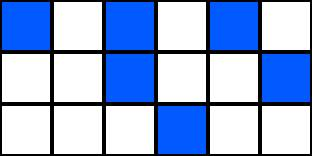
\includegraphics[scale=0.9]{pauta.jpg}
\caption{Exemplo de uma imagem da matriz representativa.}
\label{img.expauta}
\end{figure}

\chapter{Testes}
\label{chap.tests}

Para garantir o bom funcionamento do programa, foram efectuados diversos testes unitários aos diferentes programas.

Na criação, foram testados os efeitos que podem ser adicionados aos excertos. Como as funções de efeitos recebem listas de \textit{frames}, para as testar, forneceram-se listas de poucos valores estratégicos de modo a garantir aspectos como o comportamento das funções com listas vazias ou com valores iguais. Testaram-se, ainda, as funções linear e módulo, testando com abcissas nos extremos do intervalo e valores médios.

No que toca a testes unitários ao acesso à base de dados, foram efetuados testes à integridade das \textit{queries} de \textit{get}. Todas as funções deste tipo foram testadas, sendo as mais gerais (como \textbf{getSamples()}, \textbf{getSongs()}, que são as funções sem argumentos e \textbf{getEffects()}) apenas para o caso de existir um erro interno na base de dados, sendo que o \textit{output} irá ser sempre muito variável, dependendo dos dados que forem introduzidos. Para o resto das funções, averigou-se algumas variações entre parâmetros, e parâmetros que não irão ser geralmente enviados, ou que retornem erros previsíveis (como \textbf{ELEMENT\_NOT\_EXISTENT} ou \textbf{PARAM\_ERROR} ). Da inserção de parâmetros válidos nestes testes, esperam-se \textit{outputs} previsíveis.

\chapter{Conclusões}
\label{chap.conclusao}

Todas as funcionalidades pedidas funcionam e os testes unitários passam sem erros.

\subsubsection{Divisão do Trabalho}

\begin{itemize}
	\item \textbf{Rodrigo Rosmaninho} - \textbf{25\%}
		\begin{itemize}
			\item Aplicação Web (CherryPy - api.py)
			\item JavaScript das páginas de lista de músicas e excertos
			\item Ajuda na base de dados
			\item Ajuda nas páginas HTML e create.js
		\end{itemize}
	\item \textbf{Eurico Dias} - \textbf{25\%}
		\begin{itemize}
			\item Script de criação da base de dados (proj2db.sql)
			\item Funções python de leitura e escrita na base de dados (db.py)
			\item Gerador de imagens (genImage.py)
			\item Ajuda na aplicação web (CherryPy - api.py)
		\end{itemize}
	\item \textbf{João Trindade} - \textbf{25\%}
		\begin{itemize}
			\item Páginas HTML
			\item CSS (main.css)
			\item Ajuda no Javascript
		\end{itemize}
	\item \textbf{Pedro Valério} - \textbf{25\%}
		\begin{itemize}
			\item Gerador de Músicas (Sound.py)
			\item Javascript da página de geração de músicas
			\item Função de tratar e guardar informação da música na DB
			\item Ajuda na página HTML create.html
		\end{itemize}

\end{itemize}

%%%%%%%%%%%%%%%%%%%%%%%%%%%%%%%%%
\chapter*{Acrónimos}
\begin{acronym}
	\acro{wav}[WAV]{WAVEform audio file format}
	\acro{md5}[MD5]{Message-Digest algorithm 5}
	\acro{json}[JSON]{JavaScript Object Notation}
	\acro{sql}[SQL]{Structured Query Language}
	\acro{bpm}[BPM]{Beats per Minute}
\end{acronym}


%%%%%%%%%%%%%%%%%%%%%%%%%%%%%%%%%
%\printbibliography

\end{document}
